
% Spellcheck: ok
% Mikes: ok

% ============================================================
\chapter{Time As a Variable: Time-Series Analysis}{}{}
\label{ch:timeseries}

\index{time-series analysis|(} 
\index{data analysis!time-series analysis|(}
 
\Fint{If we follow the variation of some quantity over time, we are
dealing with a \emph{time series}. Time} series are incredibly common:
examples range from stock market movements to the tiny icon that
constantly displays the CPU utilization of your desktop computer for the
previous 10 seconds. What makes time series so common and so important is
that they allow us to see not only a single quantity by itself but at
the same time give us the typical ``context'' for this quantity. Because
we have not only a single value but a bit of history as well, we can
recognize any changes from the typical behavior particularly easily.

On the face of it, time-series analysis is a bivariate problem (see
Chapter \ref{ch:bivariate}). Nevertheless, we are dedicating a
separate chapter to this topic.  Time series raise a different set of
issues than many other bivariate problems, and a rather specialized
set of methods has been developed to deal with them.

% ============================================================
\section{Examples}

\index{time-series analysis!examples|(} 

To get started, let's look at a few different time series to develop a
sense for the scope of the task.

% The \mathrm{} stuff comes from the LaTeX Guide, p144 (bottom)

Figure \ref{fig:co2hawaii} shows the concentration of carbon dioxide
($\mathrm{CO_2}$) in the atmosphere, as measured by the observatory on
Mauna Loa on Hawaii, recorded at monthly intervals since 1959.
% over the years 1959 through 1990.

This data set shows two features we often find in a time-series plot:
trend and seasonality. There is clearly a steady, long-term growth in
the overall concentration of $\mathrm{CO_2}$; this is the
\emph{trend}. \index{trends!time-series} In addition, there is also a regular periodic pattern;
this is the \emph{seasonality}. \index{seasonality!time-series}  If we look closely, we see that the
period in this\vadjust{\pagebreak} case is exactly 12 months, but we will
use the term ``seasonality'' for any regularly recurring feature,
regardless of the length of the period. We should also note that the
trend, although smooth, does appear to be nonlinear, and in itself may be
changing over time.
% an (in fact, the growth in $\mathrm{CO_2}$ concentration seems 
% to be accelerating).

\begin{figure}
    \centerline{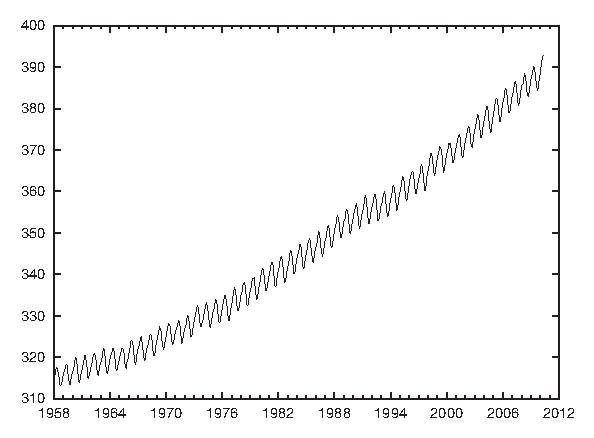
\includegraphics{img/co2hawaii}}
  \caption{Trend and seasonality: the concentration of CO$_2$
    (in parts per million) in the atmosphere as measured by the
    observatory on Mauna Loa, Hawaii, at monthly intervals.}
  \label{fig:co2hawaii}
\end{figure}

Figure \ref{fig:gasfurnace} displays the concentration of a certain
gas in the exhaust of a gas furnace over time. In many ways, this
example is the exact opposite of the previous example. Whereas the
data in Figure \ref{fig:co2hawaii} showed a lot of regularity and a
strong trend, the data in Figure \ref{fig:gasfurnace} shows no trend but
a lot of noise.

\begin{figure}
  \centerline{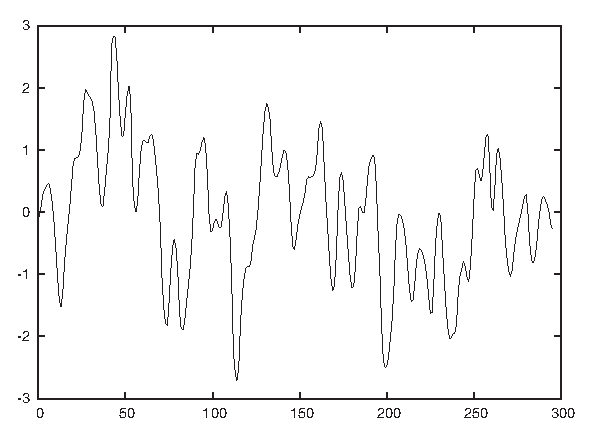
\includegraphics{img/gasfurnace}}
  \caption{No trend but relatively smooth variation over time:
    concentration of a certain gas in a furnace exhaust (in arbitrary
    units).}  
  \label{fig:gasfurnace}
\end{figure}

Figure \ref{fig:phonecost} shows the dramatic drop in the cost of a
typical long-distance phone call in the U.S.\ over the last century.
The strongly nonlinear trend is obviously the most outstanding feature
of this data set. As with many growth or decay processes, we may
suspect an exponential time development; in fact, in a
semi-logarithmic plot (Figure \ref{fig:phonecost}, inset) the data
follows almost a straight line, confirming our expectation. Any
analysis that fails to~account explicitly for this behavior of the
original data is likely to lead us astray. We should therefore work
with the logarithms of the cost, rather than with the absolute\break cost.

\begin{figure}
  \centerline{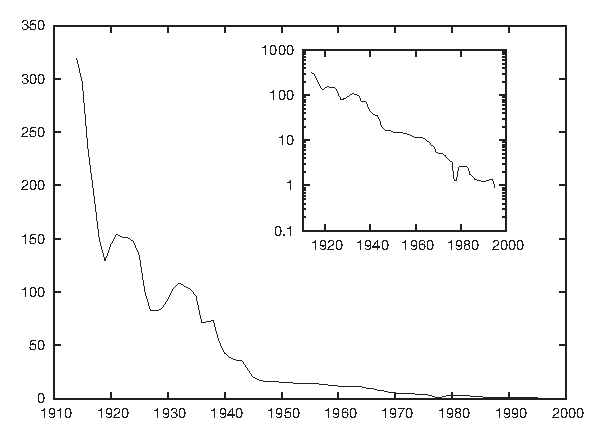
\includegraphics{img/phonecost}}
  \caption{Nonlinear trend: cost of a typical long-distance phone call
    in the U.S.}
  \label{fig:phonecost}
\end{figure}

There are some additional questions that we should ask when dealing
with a long-running data set like this.  What exactly is a ``typical''
long-distance call, and has that definition changed over the
observation period?  Are the costs adjusted for inflation or not? The
data itself also begs closer scrutiny. For instance, the
uncharacteristically low prices for a couple of years in the late
1970s make me suspicious: are they the result of a clerical error (a
typo), or are they real? Did the breakup of the AT\&T system\vadjust{\pagebreak} have
anything to do with these low prices? We will not follow up on these
questions here because I am presenting this example only as an
illustration of an exponential trend, but any serious analysis of this
data set would have to follow up on these questions.

\begin{figure}[t!]
   \centerline{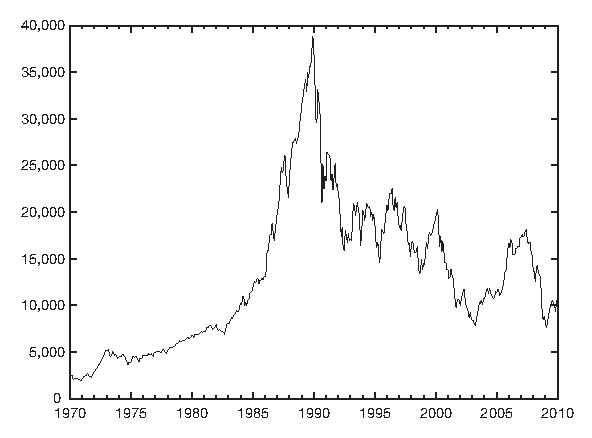
\includegraphics{img/nikkei}}
  \caption{Change in behavior: the Nikkei Stock Index over the last 
    40 years.}
  \label{fig:nikkei}
\end{figure}

Figure \ref{fig:nikkei} shows the development of the Japanese stock
market as represented by the Nikkei Stock Index over the last 40
years, an example of a time\vadjust{\pagebreak} series that exhibits a marked change in
behavior. Clearly, whatever was true before the New
Year's Day 1990 was no longer true afterward. (In fact, by looking
closely, you can make out a second change in behavior that was more
subtle than the bursting of the big Japanese bubble: its beginning,
sometime around 1985--1986.)

This data set should serve as a cautionary example. All time-series
analysis is based on the assumption that the processes generating the
data are stationary in time. If the rules of the game change, then
time-series analysis is the wrong tool for the task; instead we need
to investigate what caused the break in behavior. More benign examples
than the bursting of the Japanese bubble can be found: a change in
sales or advertising strategy may significantly alter a company's
sales patterns. In such cases, it is more important to inquire about
any further plans that the sales department might have, rather than to
continue working with data that is no longer representative!

After these examples that have been chosen for their ``textbook''
properties, let's look at a ``real-world'' data set. Figure
\ref{fig:callcenter} shows the number of daily calls placed to a call
center for a time period slightly longer than two years. In comparison
to the previous examples, this data set has a lot more structure,
which  makes it hard to determine even basic properties. We can see
some high-frequency variation, but it is not clear whether this is
noise or has some form of regularity to it. It is also not clear
whether there is any sort of regularity on a longer time scale.  The
amount of variation makes it hard to recognize any further structure.
For instance, we cannot tell if there is a longer-term trend in the
data. We will come back to this example later in the chapter.

\begin{figure}
  \centerline{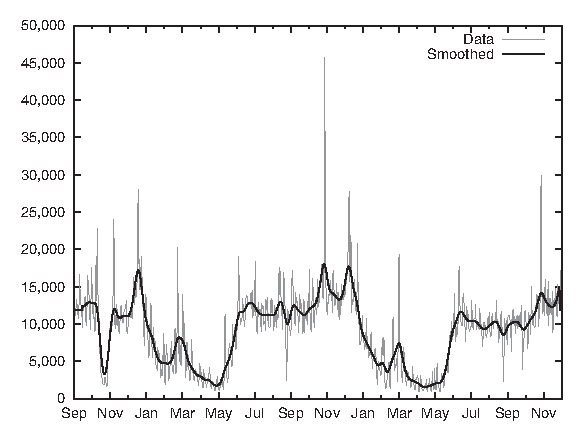
\includegraphics{img/callcenter}}
  \caption{A real-world data set: number of daily calls placed to a
    call center.  The data exhibits short- and long-term seasonality,
    noise, and possibly changes in behavior.  Also shown is the result
    of applying a 31-point Gaussian smoothing filter.}
  \label{fig:callcenter}
\end{figure}

\index{time-series analysis!examples|)} 

% ============================================================
\section{The Task}

\index{time-series analysis!components of|(} 

After this tour of possible time-series scenarios, we can identify the
main components of every time series:

\begin{itemize}
\item Trend\index{trends!time-series}
\item Seasonality\index{seasonality!time-series}
\item Noise\index{noise!time-series}
\item Other(!)
\end{itemize}

The trend may be linear or nonlinear, and we may want to investigate
its magnitude. The seasonality pattern may be either additive or
multiplicative. In the first case, the seasonal change has the same
\emph{absolute} size no matter what the magnitude of the current
baseline of the series is; in the latter case, the seasonal change has
the same \emph{relative} size compared with the current magnitude of
the series. Noise (\ie, some form of random variation) is almost
always part of a time series. Finding ways to reduce the noise in the
data is usually a significant part of the analysis process. Finally,
``other'' includes anything else that we may observe in a time series,
such as particular significant changes in overall behavior, special
outliers, missing data---anything remarkable at all.

Given this list of components, we can summarize what it means to
``analyze'' a time series. We can distinguish three basic tasks:

\begin{itemize}
\item Description
\item Prediction
\item Control
\end{itemize}

Description attempts to identify components of a time series (such as
trend and seasonality or abrupt changes in behavior). Prediction seeks
to forecast future values.  Control in this context means the
monitoring of a process over time with the purpose of keeping it
within a predefined band of values---a typical task in many
manufacturing or engineering environments. We can distinguish the
three tasks in terms of the time frame they address: description looks
into the past, prediction looks to the future, and control
concentrates on the present.\vspace*{-9pt}


\subsection{Requirements and the Real World}

Most standard methods of time-series analysis make a number of
assumptions about the underlying data.

\begin{itemize}
\item Data points have been taken at equally spaced time steps, with
  no missing data points.

\item The time series is sufficiently long (50 points are often 
  considered as an absolute minimum).

\item The series is \emph{stationary}: it has no trend, no
  seasonality, and the character (amplitude and frequency) of any
  noise does not change with time.
\end{itemize}

Unfortunately, most of these assumptions will be more or less violated
by any real-world data set that you are likely to encounter. Hence you
may have to perform a certain amount of data cleaning before you can
apply the methods described in this chapter.

If the data has been sampled at irregular time steps or if some of the
data points are missing, then you can try to interpolate the data and
resample it at equally spaced intervals. Time series obtained from
electrical systems or scientific experiments can be almost arbitrarily
long, but most series arising in a business context will be quite
short and contain possibly no more than two dozen data points. The
exponential smoothing methods introduced in the next section are
relatively robust even for relatively short series, but somewhere
there is a limit. Three or four data points don't constitute a series!
Finally, most interesting series will not be stationary in the sense
of the definition just given, so we may have to identify and remove
trend and seasonal components explicitly (we'll discuss how to do that
later). Drastic changes in the nature of the series also violate the
stationarity condition. In such cases we must not continue blindly but
instead deal with the break in the data---for example, by treating the
data set as two different series (one before and one after the event). 

\index{time-series analysis!components of|)} 

% ============================================================
\section{Smoothing}

\index{time-series analysis!smoothing|(}
\index{smoothing!time-series analysis|(}
  
An important aspect of most time series is, the presence of
\emph{noise}---that is, random (or apparently random) changes in the
quantity of\vadjust{\pagebreak} interest. Noise occurs in many real-world data sets, but
we can often reduce the noise by improving the apparatus used to
measure the data or by collecting a larger sample and averaging over
it. But the particular structure of time series makes this impossible:
the sales figures for the last 30 days are fixed, and they constitute
all the data we have. This means that removing noise, or at least
reducing its influence, is of particular importance in time-series
analysis. In other words, we are looking for ways to \emph{smooth} the
signal.


\begin{figure}
  \centerline{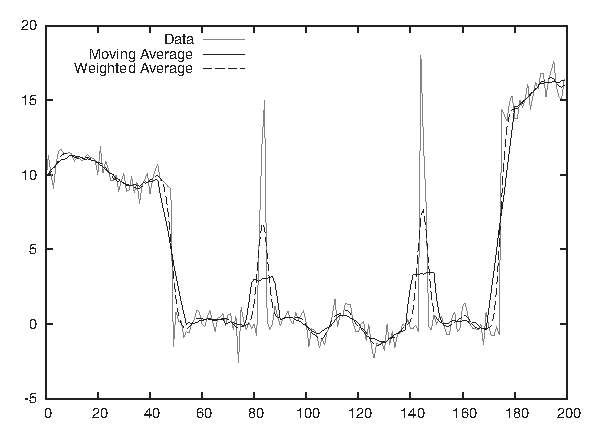
\includegraphics{img/runningavg}}
  \caption{Simple and a Gaussian weighted moving average: the weighted
    average is less affected by sudden jumps in the data.}
  \label{fig:runningavg}
\end{figure}

\subsection{Running Averages}

\index{running averages}
 
The simplest smoothing algorithm that we can devise is the
\emph{running}, \emph{moving}, or \emph{floating average}.\index{moving averages}\index{floating averages} The
idea is straightforward: for any odd number of consecutive points, replace the
centermost value with the average of the other points (here, the
$\braces{x_i}$ are the data points and the smoothed value at position
$i$ is $s_i$):
%
% x_i \rightarrow x_i = \frac{1}{2k+1} \sum_{j=-k}^k x_{i+j}
\[ 
s_i = \frac{1}{2k+1} \sum_{j=-k}^k x_{i+j}
\]
%
This naive approach has a serious problem, as you can see in Figure
\ref{fig:runningavg}. The figure shows the original signal together
with the 11-point moving average. Unfortunately, the signal has some
sudden jumps and occasional large ``spikes,'' and we can see how the
smoothed curve is affected by these events: whenever a spike enters
the smoothing window, the moving average is abruptly distorted by the
single, uncommonly large value until the outlier leaves the smoothing
window again---at which point the floating average equally abruptly
drops again.



We can avoid this problem by using a \emph{weighted moving average},\index{weighted moving averages} 
which places less weight on the points at the edge of the smoothing
window. Using such a weighted average, any new point that enters the
smoothing window is only gradually added to the average and then
gradually removed again:
%
% x_i \rightarrow x_i = \sum_{j=-k}^k w_j x_{i+j}
% \quad \text{ where } \sum_{j=-k}^k w_j = 1
\[ 
s_i = \sum_{j=-k}^k w_j x_{i+j} 
      \quad \text{where } \sum_{j=-k}^k w_j = 1
\]
%
Here the $w_j$ are the weighting factors. For example, for a 3-point
moving average, we might use $( 1/4, 1/2, 1/4 )$. The particular choice
of weight factors is not very important provided they are peaked at
the center, drop toward the edges, and add up to $1$. I like to use
the Gaussian function:\index{Gaussian distribution (Gaussian function)!moving averages}
%
\[ 
f(x,\sigma) = \frac{1}{\sqrt{2 \pi \sigma^2}} 
              \exp \paren{- \frac{1}{2} \paren{ \frac{x}{\sigma} }^2}
\]
%
to build smoothing weight factors. The parameter $\sigma$ in the
Gaussian controls the width of the curve, and the function is
essentially zero for values of $x$ larger than about $3.5 \sigma$.
Hence $f(x,1)$ can be used to build a 9-point kernel by evaluating
$f(x,1)$ at the positions $[-4,-3,-2,-1,0,1,2,3,4]$. Setting
$\sigma=2$, we can form a 15-point kernel by evaluating the Gaussian
for all integer arguments between $-7$ and $+7$. And so on.


\subsection{Exponential Smoothing}

\index{exponential smoothing|(}
 
All moving-average schemes have a number of problems.

\begin{itemize}
\item They are painful to evaluate. For each point, the calculation
  has to be performed from scratch. It is not possible to evaluate
  weighted moving averages by updating a previous result.

\item Moving averages can never be extended to the true edge of the
  available data set, because of the finite width of the averaging
  window. This is especially problematic because often it is precisely
  the behavior at the leading edge of a data set that we are most
  interested in.

\item Similarly, moving averages are not defined \emph{outside} the
  range of the existing data set.  As a consequence, they are of no
  use in forecasting.
\end{itemize}

Fortunately, there exists a very simple calculational scheme that
avoids all of these problems. It is called \emph{exponential
  smoothing} or \emph{Holt--Winters method}. There are various forms
of exponential smoothing: single exponential smoothing for series that
have neither trend nor seasonality, double exponential smoothing for
series exhibiting a trend but no seasonality, and triple exponential
smoothing for series with both trend and seasonality.  The term
``Holt--Winters method'' is sometimes reserved for triple exponential
smoothing alone.

All exponential smoothing methods work by updating the result from the
previous time step using the new information contained in the data of
the current time step. They do so by ``mixing'' the new information
with the old one, and the relative weight of old and new information
is controlled by an adjustable mixing parameter. The various methods
differ in terms of the number of quantities they track and the
corresponding number of mixing parameters.

The recurrence relation for single exponential smoothing is
particularly simple:
%
\[
s_i = \alpha x_i + (1-\alpha) s_{i-1} \quad \text{with $0 \le \alpha \le 1$}
\] 
%
Here $s_i$ is the smoothed value at time step $i$, and $x_i$ is the
actual (unsmoothed) data at that time step. You can see how $s_i$ is a
mixture of the raw data and the previous smoothed value $s_{i-1}$.
The mixing parameter $\alpha$ can be chosen anywhere between $0$ and
$1$, and it controls the balance between new and old information: as
$\alpha$ approaches $1$, we retain only the current data point (\ie,
the series is not smoothed at all); as $\alpha$ approaches $0$, we
retain only the smoothed past (\ie, the curve is totally flat).

Why is this method called ``exponential'' smoothing? To see this,
simply expand the recurrence relation:
%
\begin{align*}
  s_i & = \alpha x_i + ( 1 - \alpha ) s_{i-1} \\
      & = \alpha x_i + ( 1 - \alpha ) 
          \left[ \alpha x_{i-1} + ( 1 - \alpha ) s_{i-2} \right] \\
      & = \alpha x_i + ( 1 - \alpha ) 
          \bigl[ \alpha x_{i-1} + ( 1 - \alpha ) 
          \left[ \alpha x_{i-2} + ( 1 - \alpha ) s_{i-3} \right] \bigr] \\
      & = \alpha \left[ x_i + ( 1 - \alpha ) x_{i-1} + 
          ( 1 - \alpha )^2 x_{i-2} \right] + 
          ( 1 - \alpha )^3 s_{i-3} \\
      & = \dots \\
      & = \alpha \sum_{j=0}^{i} ( 1 - \alpha )^j x_{i-j}
\end{align*}
%
What this shows is that in exponential smoothing, \emph{all} previous
observations contribute to the smoothed value, but their contribution
is suppressed by increasing powers of the parameter $\alpha$.  That
observations further in the past are suppressed multiplicatively is
characteristic of exponential behavior.  In a way, exponential
smoothing is like a floating average with infinite memory but with
exponentially falling weights. (Also observe that the sum of the
weights, $\sum_j \alpha ( 1 - \alpha )^j$, equals $1$ as required by
virtue of the geometric series $\sum_i q^i = 1/(1-q)$ for $q < 1$. See
Appendix \ref{app:calculus} for information on the geometric series.)

The results of the simple exponential smoothing procedure can be
extended beyond the end of the data set and thereby used to make a
forecast. The forecast is extremely simple:
%
\[
x_{i+h} = s_i
\]
%
where $s_i$ is the last calculated value. In other words, single
exponential smoothing yields a forecast that is absolutely flat for
all times.

Single exponential smoothing as just described works well for time
series without an overall trend. However, in the presence of an
overall trend, the smoothed values tend to lag behind the raw data
unless $\alpha$ is chosen to be close to $1$; however, in this case
the resulting curve is not sufficiently smoothed.

Double exponential smoothing \index{double exponential smoothing} corrects for this shortcoming by
retaining explicit information about the trend. In other words, we
maintain and update the state of two quantities: the smoothed signal
\emph{and} the smoothed trend. There are two equations and two mixing
parameters:\vspace*{-6pt}
%
\begin{align*}
  s_i & = \alpha x_i + ( 1 - \alpha ) ( s_{i-1} + t_{i-1} ) \\
  t_i & = \beta ( s_i - s_{i-1} ) + ( 1 - \beta ) t_{i-1}
\end{align*}\vskip-3pt
%

\noindent Let's look at the second equation first. This equation describes the
smoothed trend. The current unsmoothed ``value'' of the trend is
calculated as the difference between the current and the previous
smoothed signal; in other words, the current trend tells us how much
the smoothed signal changed in the last step. To form the smoothed
trend, we perform a simple exponential smoothing process on the trend,
using the mixing parameter $\beta$. To obtain the smoothed signal, we
perform a similar mixing as before but consider not only the previous
smoothed signal but take the trend into account as well.  The last
term in the first equation is the best guess for the current smoothed
signal---assuming we followed the previous trend for a single time
step.

%\enlargethispage{6pt}

To turn this result into a forecast, we take the last smoothed value
and, for each additional time step, keep adding the last smoothed
trend to it:\vspace*{-3pt}
%
\[
x_{i+h} = s_i + h \, t_i
\]\vskip-6pt

Finally, for triple exponential smoothing \index{triple exponential smoothing} we add yet a third quantity,
which describes the seasonality. We have to distinguish between
additive and multiplicative seasonality. For the additive case, the
equations are:\vspace*{-3pt}
%
\begin{align*}
  s_i & = \alpha ( x_i - p_{i-k} ) + ( 1 - \alpha ) ( s_{i-1} + t_{i-1} ) \\
  t_i & = \beta ( s_i - s_{i-1} ) + ( 1 - \beta ) t_{i-1} \\
  p_i & = \gamma ( x_i - s_i ) + ( 1 - \gamma ) p_{i-k} \\
  x_{i+h} & = s_i + h \, t_i + p_{i-k+h}
\end{align*}
%
For the multiplicative case, they are:\vspace*{-3pt}
%
\begin{align*}
  s_i & = \alpha \frac{x_i}{p_{i-k}} + ( 1 - \alpha ) ( s_{i-1} + t_{i-1} ) \\
  t_i & = \beta ( s_i - s_{i-1} ) + ( 1 - \beta ) t_{i-1} \\
  p_i & = \gamma \frac{x_i}{s_i} + ( 1 - \gamma ) p_{i-k} \\
  x_{i+h} & = (s_i + h \, t_i) p_{i-k+h}
\end{align*}
%

\noindent Here, $p_i$ is the ``periodic'' component, and $k$ is the length of the
period. I have also included the expressions for forecasts.

All exponential smoothing methods are based on recurrence relations.\index{recurrence relations, exponential smoothing}
This means that we need to fix the start-up values in order to use
them.  Luckily, the specific choice for these values is not very
critical: the exponential damping implies that all exponential
smoothing methods have a short ``memory,'' so that after only a few
steps, any influence of the initial values is greatly diminished. Some
reasonable choices for start-up values are:
%
\[
s_0 = x_0  
\qquad \text{or} \qquad
s_0 = \frac{1}{n} \sum_i^n x_i \quad \text{with $1 < n < 5, \dots, 10$}
\]
%
and:
%
\[
t_0 = 0 
\qquad \text{or} \qquad
t_0 = x_1 - x_0
\]

For triple exponential smoothing we must provide one full season of
values for start-up, but we can simply fill them with $1$s (for the
multiplicative model) or $0$s (for the additive model). Only if the
series is short do we need to worry seriously about finding good
starting values.

The last question concerns how to choose the mixing parameters
$\alpha$, $\beta$, and $\gamma$. My advice is trial and error. Try a
few values between $0.2$ and $0.4$ (very roughly), and see what results
you get.  Alternatively, you can define a measure for the error
(between the actual data and the output of the smoothing algorithm),
and then use a numerical optimization routine to minimize this error
with respect to the parameters. In my experience, this is usually more
trouble than it's worth for at least the following two reasons. The
numerical optimization is an iterative process that is not guaranteed
to converge, and you may end up spending way too much time coaxing the
algorithm to convergence. Furthermore, any such numerical optimization
is slave to the expression you have chosen for the ``error'' to be
minimized. The problem is that the parameter values minimizing that
error may not have some other property you want to see in your
solution (\eg, regarding the balance between the accuracy of the
approximation and the smoothness of the resulting curve) so that, in
the end, the manual approach often comes out ahead. However, if you
have many series to forecast, then it may make sense to expend the
effort and build a system that can determine the optimal parameter
values automatically, but it probably won't be easy to really make
this work.

Finally, I want to present an example of the kind of results we can
expect from exponential smoothing. Figure \ref{fig:airtraffic} is a
classical data set that shows the monthly number of international
airline passengers (in thousands of passengers).\footnote{This data is
  available in the ``airpass.dat'' data set from R.\ J.\ Hyndman's
  Time Series Data Library at \url{http://www.robjhyndman.com/TSDL}.}
The graph shows the actual data together with a triple exponential
approximation. The years 1949 through 1957 were used to ``train'' the
algorithm, and the years 1958 through 1960 are forecasted.  Note how
well the forecast agrees with the actual data---especially in  
light of the strong seasonal pattern---for a rather long forecasting
time frame (three full years!). Not bad for a method as simple as
this.

\begin{figure}
  \centerline{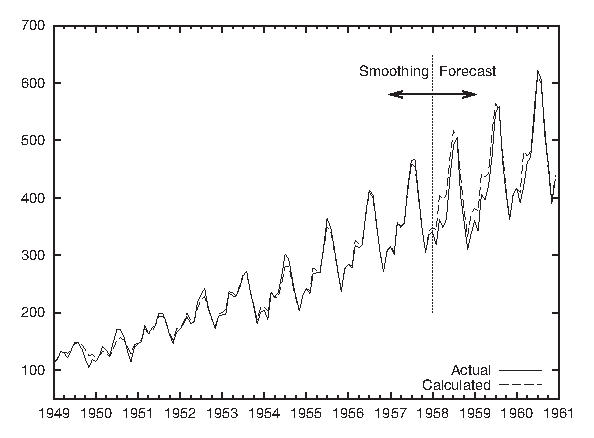
\includegraphics{img/airtraffic}}
  \caption{Triple exponential smoothing in action: comparison between
    the raw data (solid line) and the smoothed curve (dashed). For the
    years after 1957, the dashed curve shows the forecast calculated
    with only the data available in 1957.}
  \label{fig:airtraffic}
\end{figure}

\index{exponential smoothing|)}
\index{time-series analysis!smoothing|)}
\index{smoothing!time-series analysis|)}

\section{Don't Overlook the Obvious!}

On a recent consulting assignment, I was discussing monthly sales
numbers with the client when he made the following comment: ``Oh,
yes, sales for February are always somewhat lower---that's an
after effect of the Christmas peak.'' Sales are always lower in
\emph{February}? How interesting.

Sure enough, if you plotted the monthly sales numbers for the last few
years, there was a rather visible dip from the overall trend every
February. But in contrast, there wasn't much of a Christmas spike!
(The client's business was not particularly seasonal.) So why should
there be a corresponding dip two months later?

By now I am sure you know the answer already: February is
\emph{shorter} than any of the other months. And it's not a small
effect, either: with 28 days, February is about three days shorter than
the other months (which have 30--31 days). That's about 10
percent---close to the size of the dip in the client's sales numbers.

When monthly sales numbers were normalized by the number of days in
the month, the February dip all but disappeared, and the \emph{adjusted}
February numbers were perfectly in line with the rest of the months.
(The average number of days per month is $365/12 = 30.4$.)

Whenever you are tracking aggregated numbers in a time series (such as
weekly, monthly, or quarterly results), make sure that you have
adjusted for possible variation in the aggregation time frame. Besides
the numbers\vadjust{\pagebreak} of days in the month, another likely candidate for hiccups
is the number of \emph{business days} in a month (for months with five
weekends, you can expect a 20 percent drop for most business metrics).  But
the problem is, of course, much more general and can occur whenever you
are reporting aggregate \emph{numbers} rather than \emph{rates}. (If
the client had been reporting average sales per day for each month,
then there would never have been an anomaly.)

This specific problem (\ie, nonadjusted variations in aggregation
periods) is a particular concern for all business reports and
dashboards. Keep an eye out for it!


% ============================================================
\section{The Correlation Function}

\index{time-series analysis!correlation function|(} 
\index{correlation function|(}
 
The \emph{autocorrelation function} \index{autocorrelation function} is the primary diagnostic tool for
time-series analysis. Whereas the smoothing methods that we have
discussed so far deal with the raw data in a very direct way, the
correlation function provides us with a rather different view of the
same data. I will first explain how the autocorrelation function is
calculated and will then discuss what it means and how it can be used.

The basic algorithm works as follows: start with two copies of the
data set and subtract the overall average from all values.  Align the
two sets, and multiply the values at corresponding time steps with each
other. Sum up the results for all time steps. The result is the
(unnormalized) correlation coefficient at \emph{lag} $0$.  Now shift
the two copies against each other by a single time step.  Again
multiply and sum: the result is the correlation coefficient at lag
$1$. Proceed in this way for the entire length of the time series.
The set of all correlation coefficients for all lags is the
autocorrelation function. Finally, divide all coefficients by the
coefficient for lag $0$ to normalize the correlation function, so that
the coefficient for lag $0$ is now equal to $1$.

All this can be written compactly in a single formula for $c(k)$---that
is the correlation function at lag $k$:
%
\[
c(k) = \frac{\sum\limits_{i=1}^{N-k} (x_i - \mu)(x_{i+k} - \mu)}
            {\sum\limits_{i=1}^N (x_i - \mu)^2}
\qquad \text{with } \mu = \frac{1}{N} \sum_{i=1}^N x_i
\]
%
Here, $N$ is the number of points in the data set. The formula follows
the mathematical convention to start indexing sequences at $1$,
rather than the programming convention to start indexing at $0$.
Notice that we  have subtracted the overall average $\mu$ from all
values and that the denominator is simply the expression of the
numerator for lag $k=0$. Figure~\ref{fig:correlationlags} illustrates
the process.


\begin{figure}
 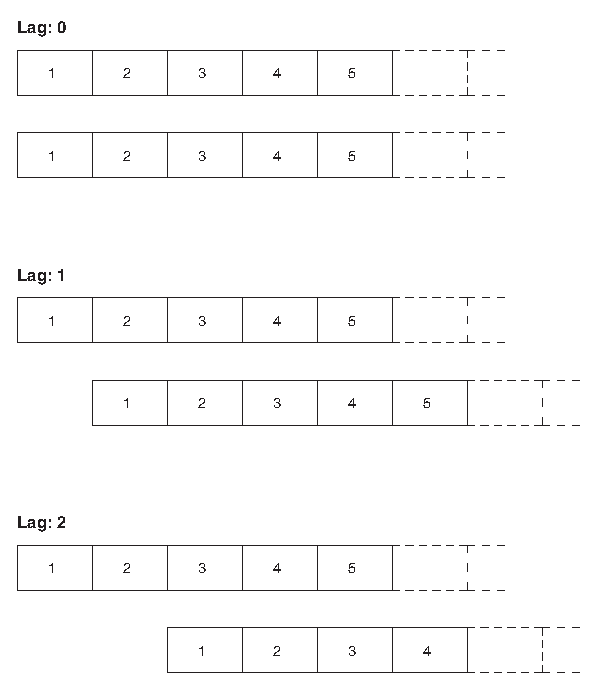
\includegraphics[scale=0.8]{img/correlationlags}
 \caption{Algorithm to compute the correlation function.}
 \label{fig:correlationlags}\vspace*{15pt}
\end{figure}

The meaning of the correlation function should be clear. Initially,
the two signals are perfectly aligned and the correlation is $1$.
Then, as we shift the signals against each other, they slowly move out
of phase with each\vadjust{\pagebreak} other, and the correlation drops. How quickly it
drops tells us how much ``memory'' there is in the data. If the
correlation drops quickly, we know that, after a few steps, the signal
has lost all memory of its recent past. However, if the correlation
drops slowly, then we know that we are dealing with a process that is
relatively steady over longer periods of time. It is also possible
that the correlation function first drops and then rises again to form
a second (and possibly a third, or fourth$,\dots$) peak. This tells us
that the two signals align again if we shift them far enough---in
other words, that there is periodicity (\ie, seasonality) in the data
set. The position of the secondary peak gives us the number of time
steps per season.

\vspace*{6pt}
\subsection{Examples}
Let's look at a couple of examples. Figure \ref{fig:gasfurnacecorr}
shows the correlation function of the gas furnace data in Figure
\ref{fig:gasfurnace}. This is a fairly typical correlation function
for a time series that has only short time correlations: the
correlation falls quickly, but not immediately, to zero. There is no
periodicity; after the initial drop, the correlation function does not
exhibit any further significant\vadjust{\vfill\pagebreak} peaks.





\begin{figure}
    \centerline{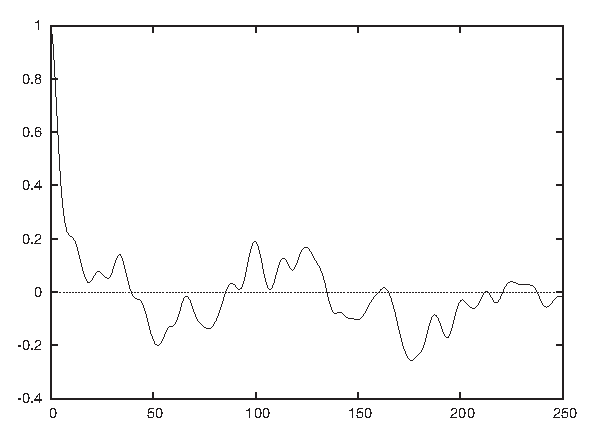
\includegraphics{img/gasfurnacecorr}}
  \caption{The correlation function for the exhaust gas data shown in
    Figure \ref{fig:gasfurnace}. The data has only short time
    correlations and no seasonality; the correlation function falls
    quickly (but not immediately) to zero, and there are no secondary
    peaks.}
  \label{fig:gasfurnacecorr}
\end{figure}

Figure \ref{fig:callcentercorr} is the correlation function for the
call center data from Figure \ref{fig:callcenter}. This data set shows
a very different behavior. First of all, the time series has a much
longer ``memory'': it takes the correlation function almost 100 days
to fall to zero, indicating that the frequency of calls to the call
center changes more or less once per quarter but not more frequently.
The second notable feature is the pronounced secondary peak at a lag
of 365 days. In other words, the call center data is highly seasonal
and repeats itself on a yearly basis.  The third feature is the small
but regular sawtooth structure. If we look closely, we will find that
the first peak of the sawtooth is at a lag of 7 days and that all
repeating ones occur at multiples of 7. This is the signature of the
high-frequency component that we could see in Figure
\ref{fig:callcenter}: the traffic to the call center exhibits a
secondary seasonal component with 7-day periodicity. In other words,
traffic is weekday dependent (which is not too surprising).

\begin{figure}
  \centerline{ 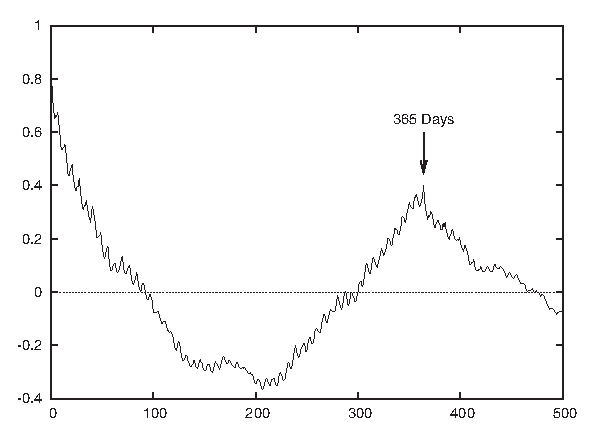
\includegraphics{img/callcentercorr}}
  \caption{The correlation function for the call center data shown in
    Figure \ref{fig:callcenter}. There is a secondary peak after
    exactly 365 days, as well as a smaller weekly structure to the
    data.}
  \label{fig:callcentercorr}
\end{figure}


\subsection{Implementation Issues}

So far I have talked about the correlation function mostly from a
conceptual point of view. If we want to proceed to an actual
implementation, there are some fine points we need to worry about.

The autocorrelation function \index{autocorrelation function} is intended for time series that do not
exhibit a trend \index{trends!time-series} and have zero mean. Therefore, if the series we want
to analyze does contain a trend, then we must remove it first. There
are two ways to do this: we can either subtract the trend or we can
difference the series.

Subtracting the trend is straightforward---the only problem is that we
need to determine the trend first! Sometimes we may have a ``model''
for the expected behavior and can use it to construct an explicit
expression for the trend.  For instance, the airline passenger data
from the previous section, describes a growth process, and so we should
suspect an exponential trend ($a \exp(x/b)$).  We can now try guessing
values for the two parameters and then subtract the exponential term
from the data. For other data sets, we might try a linear or power-law
trend, depending on the data set and our understanding of the process
generating the data. Alternatively, we might first apply a smoothing
algorithm to the data and then subtract the result of the smoothing
process from the raw data. The result will be the trend-free ``noise''
component of the time series.

A different approach consists of \emph{differencing} \index{differencing, time-series} the series:
instead of dealing with the raw data, we instead work with the
\emph{changes} in the data from one time step to the next.
Technically, this means replacing the original series $x_i$ with one
consisting of the differences of consecutive elements: $x_{i+1} -
x_i$. This process can be repeated if necessary, but in most cases,
single differencing is sufficient to remove the trend entirely.

Making sure that the time series has zero mean is easier: simply
calculate the mean of the (de-trended!) series and subtract it before
calculating the correlation function.  This is done explicitly in the
formula for the correlation function  given earlier.

Another technical wrinkle concerns how we implement the sum in the
formula for the numerator. As written, this sum is slightly messy,
because its upper limit depends on the lag.  We can simplify the
formula by \emph{padding} one of the data sets with $N$ zeros on the
right and letting the sum run from $i=1$ to $i=N$ for all\vadjust{\pagebreak} lags. In
fact, many computational software packages assume that the data has
been prepared in this way (see the Workshop section in this chapter).

The last issue you should be aware of is that there are two different
normalization conventions for the autocorrelation function, which are
both widely used. In the first variant, numerator and denominator are
not normalized separately---this is the scheme used in the previous
formula.  In the second variant, the numerator and denominator are
each normalized by the number of nonzero terms in their respective
sum.  With this convention, the formula becomes:
%
\[
c(k) = \frac{ \dfrac{1}{N-k} \sum\limits_{i=1}^{N-k} 
                                        (x_i - \mu)(x_{i+k} - \mu) }
            { \dfrac{1}{N} \sum\limits_{i=1}^N (x_i - \mu)^2 }
       \qquad \text{with } \mu = \frac{1}{N} \sum_{i=1}^N x_i
\]
%
Both conventions are fine, but if you want to compare results from
different sources or different software packages, then you will have
to make sure you know which convention each of them is following!\vspace*{-9pt}

\index{time-series analysis!correlation function|)} 
\index{correlation function|)}

% ============================================================
\section{Optional: Filters and Convolutions}

\index{time-series analysis!filters and convolutions}
\index{filters, time-series analysis}
\index{convolutions, time-series analysis}  
 
Until now we have always spoken of time series in a direct fashion,
but there is also a way to describe them (and the operations performed
on them) on a much higher level of abstraction. For this, we borrow
some concepts and terminology from electrical engineering,
specifically from the field of digital signal processing (DSP).\index{DSP (digital signal processing)} \index{digital signal processing (DSP)} 

In the lingo of DSP, we deal with \emph{signals} (time series)\index{signals, DSP} and
\emph{filters} (operations). Applying a filter to a signal produces a
new (filtered) signal. Since filters can be applied to any signal, we
can apply another filter to the output of the first and in this way
chain filters together (see Figure \ref{fig:filterchain}).  Signals
can also be combined and subtracted from each other.

\begin{figure}
  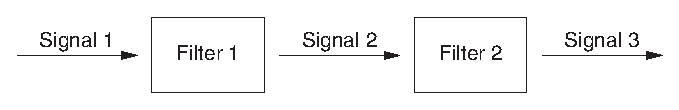
\includegraphics{img/filterchain}
  \caption{A filter chain: each filter applied to a signal yields another
    signal, which itself can be filtered.}
  \label{fig:filterchain}\vspace*{-9pt}
\end{figure} 

As it turns out, many of the operations we have seen so far
(smoothing, differencing) can be expressed as filters. We can
therefore use the convenient high-level language of DSP when
referring to the processes of time-series analysis. To make this
concrete, we need to understand how a filter is represented and what
it means to ``apply'' a filter to a signal.

Each digital filter is represented by a set of coefficients or
weights. To apply the filter, we multiply the coefficients with a subset
of the signal. The sum of the products is the value of the resulting
(filtered) signal:
%
\[
y_t = \sum_{i=-k}^k w_i x_{t+i}
\]
%
\clearpage

\noindent
This should look familiar! We used a similar expression when talking
about moving averages earlier in the chapter. A moving average is
simply a time series run through an $n$-point filter, where every
coefficient is equal to $1/n$. A weighted moving average filter
similarly consists of the weights used in the expression for the
average.

The filter concept is not limited to smoothing operations. The
differencing step discussed in the previous section can be viewed as
the application of the filter $[1, -1]$. We can even shift an entire
time series forward in time by using the filter $[0, 1]$.

The last piece of terminology that we will need concerns the peculiar
sum of a product that we have encountered several times by now.  It's
called a \emph{convolution}. A convolution is a way to combine two
sequences to yield a third sequence, which you can think of as
the ``overlap'' between the original sequences. The convolution
operation is usually defined as follows:
%
\[
y_t = \sum_{i=-\infty}^\infty w_i x_{t-i}
\]
%
Symbolically, the convolution operation is often expressed through an
asterisk: $y = w \star x$, where $y$, $w$, and $x$ are sequences.

Of course, if one or both of the sequences have only a finite number
of elements, then the sum also contains only a finite number of terms
and therefore poses no difficulties. You should be able to convince
yourself that every application of a filter to a time series that we
have done was in fact a convolution of the signal with the filter.
This is true in general: applying a filter to a signal means forming
the convolution of the two. You will find that many numerical software
packages provide a convolution operation as a built-in function,
making filter operations particularly convenient to use.

I must warn you, however, that the entire machinery of digital signal
processing is geared toward signals of infinite (or almost infinite)
length, which makes good sense for typical electrical signals (such as
the output from a microphone or a radio receiver). But for the rather
short time series that we are likely to deal with, we need to pay
close attention to a variety of \emph{edge effects}.  For example, if
we apply a smoothing or differencing filter, then the resulting series
will be shorter, by half the filter length, than the original series.
If we now want to subtract the smoothed from the original signal, the
operation will fail because the two signals are not of equal length.
We therefore must either pad the smoothed signal or truncate the
original one. The constant need to worry about padding and proper
alignment detracts significantly from the conceptual beauty of the
signal-theoretic approach when used with time series of relatively
short duration. 

% ============================================================
\section{Workshop: scipy.signal}

\index{time-series analysis!scipy.signal|(}
\index{scipy.signal|(}  

The \texttt{scipy.signal} package provides functions and operations
for digital signal processing that we can use to good effect to
perform calculations\vadjust{\pagebreak} for time-series analysis. The
\texttt{scipy.signal} package makes use of the signal processing
terminology introduced in the previous section.

The listing that follows shows all the commands used to create graphs
like Figures \ref{fig:callcenter} and \ref{fig:callcentercorr},
including the commands required to write the results to file. The code
is heavily commented and should be easy to understand.

\begin{verbatim}
from scipy import *
from scipy.signal import *
from matplotlib.pyplot import *

filename = 'callcenter'


# Read data from a text file, retaining only the third column.
# (Column indexes start at 0.)
# The default delimiter is any whitespace.
data = loadtxt( filename, comments='#', delimiter=None, usecols=(2,) )

# The number of points in the time series. We will need it later.
n = data.shape[0]

# Finding a smoothed version of the time series:
# 1) Construct a 31-point Gaussian filter with standard deviation = 4
filt = gaussian( 31, 4 )
# 2) Normalize the filter through dividing by the sum of its elements
filt /= sum( filt )
# 3) Pad data on both sides with half the filter length of the last value
#    (The function ones(k) returns a vector of length k, with all elements 1.)
padded = concatenate( (data[0]*ones(31//2), data, data[n-1]*ones(31//2)) )
# 4) Convolve the data with the filter. See text for the meaning of "mode".
smooth = convolve( padded, filt, mode='valid' )

# Plot the raw data together with the smoothed data:
# 1) Create a figure, sized to 7x5 inches
figure( 1, figsize=( 7, 5 ) )
# 2) Plot the raw data in red
plot( data, 'r' )
# 3) Plot the smoothed data in blue
plot( smooth, 'b' )
# 4) Save the figure to file
savefig( filename + "_smooth.png" )
# 5) Clear the figure
clf()

# Calculate the autocorrelation function:
# 1) Subtract the mean 
tmp = data - mean(data)
# 2) Pad one copy of data on the right with zeros, then form correlation fct
#    The function zeros_like(v) creates a vector with the same dimensions
#    as the input vector v but with all elements zero.
corr = correlate( tmp, concatenate( (tmp, zeros_like(tmp)) ), mode='valid' )
# 3) Retain only some of the elements
corr = corr[:500]
\end{verbatim}
\begin{verbatim}
# 4) Normalize by dividing by the first element
corr /= corr[0]


# Plot the correlation function:
figure( 2, figsize=( 7, 5 ) )
plot( corr )
savefig( filename + "_corr.png" )
clf()
\end{verbatim}

The package provides the Gaussian filter as well as many others.  The
filters are not normalized, but this is easy enough to accomplish.

More attention needs to be paid to the appropriate padding and
truncating. For example, when forming the smoothed version of the
data, I pad the data on both sides by half the filter length to ensure
that the smoothed data has the same length as the original set. The
\texttt{mode} argument to the \texttt{convolve()} and
\texttt{correlate} functions determines which pieces of the resulting
vector to retain. Several modes are possible. With
\texttt{mode="same"}, the returned vector has as many elements as the
largest input vector (in our case, as the padded data vector), but the
elements closest to the ends would be corrupted by the padded values.
In the listing, I therefore use \texttt{mode="valid"}, which retains
only those elements that have full overlap between the data and the
filter---in effect, removing the elements added in the padding step.

Notice how the signal processing machinery leads in this application
to very compact code. Once you strip out the comments and plotting
commands, there are only about 10 lines of code that perform actual
operations  and calculations.  However, we had to pad all data
carefully and ensure that we kept only those pieces of the result that
were least contaminated by the padding.

\index{time-series analysis!scipy.signal|)}
\index{scipy.signal|)}  

% ============================================================
% \section{Summary}
% 
% Time series are both common and important. But because they arise in
% so many, and so many \emph{different} contexts, little can be said
% about them without knowing the details. Studying and classifying the
% nature of each time series is therefore very important --- blindly
% applying ``cook book'' methods, no matter how sophisticated, is never
% a good strategy.
% 
% The two most important tools for studying time series are the time
% plot and the plot of the auto-correlation function. Both together can
% reveal most of what can be found out about any particular time series.
% The signal theoretic methodology that we discussed briefly can provide
% a convenient framework to handle the calculations that are required.
% 
% Smoothing and forecasting are the two most often desired results of
% time series analysis and here I strongly recommend simple, yet robust
% methods, such as weighted averages (for smoothing) and exponential
% smoothing (for forecasting).

% ============================================================
\section{Further Reading}

\begin{itemize}
\item \cit{The Analysis of Time Series}{Chris Chatfield}{6th ed.,
    Chapman \& Hall}{2003}
    This is my preferred text on time-series analysis. It combines a
    thoroughly practical approach with mathematical depth and a healthy
    preference for the simple over the obscure. Highly recommended.
\end{itemize}

\index{time-series analysis|)} 
\index{data analysis!time-series analysis|)}
